\documentclass[12pt]{article}
% Packages
\usepackage{amsmath}
\usepackage[table,xcdraw]{xcolor}
\usepackage{graphicx}
\usepackage{listings}
\usepackage{float}

\begin{document}
\title{Group 7 Project Report}
\maketitle
\author{Sydney, Brandon, Maria, Daniel, Eric}\\
\date{\today}
\pagenumbering{arabic} % - gobble (no numbers) arabic (arabic numbers) roman - (roman numbers)
Test text for the report that we need to write within the new few days.
\tableofcontents{}
\listoffigures
\indent \\\\\\\\\\\\\\\\\\\\\\\\\\\\\\\\\\\\\\\\\\\\\\\\\\\\\\
	\section{Part 1: Comparison of Sorting Algorithms}
	The efficient method of finding all the pairs/elements equal to the sum.
	\subsection{1. Theoretical question}
	Insertion Sort:\\
	
	Best Case: O(n) - Sorted Array\\
	\indent Average Case: O($n^2$) - Random Order Array\\
	\indent Worst Case: O($n^2$) - Reversed Array\\
	
	Regarding Insertion Sort, the best case is achieved when the input array is in already sorted order. This is because the algorithm must do only one comparison for each element, so it must 		do n comparisons which results in a time complexity of O(n). The average case occurs when the elements in the array are in any random order. They are neither reversed nor in sorted 			order. This results in a time complexity of O($n^2$). The worst case occurs when the input array is in reverse order. This is because each element in the array must be compared with all of 			the other elements. Like the average case, this also results in a time complexity of O($n^2$).\\ 
	
	\noindent Selection Sort:\\
	
	\indent	Best Case: O($n^2$) - Sorted Array\\
	\indent	Average Case: O($n^2$) - Random Order Array\\
	\indent	Worst Case: O($n^2$) - Reversed Array\\
	
	Regarding Selection Sort, the best case, worst case, and average case all result in the same time  complexity, which is O($n^2$) . This is due to the fact that the algorithm will do (n-1) comparisons depending on the size of n. For example if n = 8, the algorithm will do (n-1) + (n-2) + (n-3) + (n-4) + (n-5) + … + 1. The algorithm also uses double nested for loops, which would explain why Selection Sort has a time complexity of O($n^2$) in all 3 cases.\\
	\\
	\\
	\\
	
	\noindent Bubble Sort:\\
	
	\indent Best Case: O(n) - Sorted Array\\
	\indent	Average Case: O($n^2$) - Random Order Array\\
	\indent	Worst Case: O($n^2$) - Reversed Array\\
	
	Regarding Bubble Sort, The best case occurs when the array is already sorted because during the first iteration of the algorithm the swap will not occur because the left element will not be greater than the right. This means that the time complexity will be O(n) because the algorithm will traverse through each element one time. Unless the array is already in sorted order the best case, worst  case, and average case will all be O($n^2$). This is because the algorithm will traverse through each element and compare it with all other elements and also swap them if left > right.\\
	
	\noindent Merge Sort:\\
	
	\indent Best Case: O(n log n) - Sorted Array\\
	\indent Average Case: O(n log n) - Random Order Array\\
	\indent Worst Case: O(n log n) - reversed Array\\
	
	Regarding Merge Sort, it is a divide and conquer algorithm, and a recurrence needs to be resolved to estimate its time consumption. In the case of Merge Sort, an important feature is that its efficiency regardless of the case (best, worst, or average) the Merge Sort will always be O(nlogn). This is because splitting the problem always generates two subproblems half the size of the original problem (2T(n/2)). The algorithm bases the ordering on successive merge runs, a routine that joins two ordered parts of an array into an ordered one. Also, it is important to remember that the merge algorithm is (O(n1 + n2) = O(n).\\
	\\
	\\
	\\
	\\
	\\
	\\
	\\
	\\
	\noindent Quick sort:\\
	
	\indent Best Case: O(nlogn)\\
	\indent Occurs when the chosen pivot splits the vector into two size subvectors\\
	\indent equal to n/2.\\
	\indent T(n) = 2T(n/2) + n – 1\\
	\indent T(1) = T(0) = 1\\
	\indent Solving (divide and conquer):\\
	\indent T(n) = O(n log n).\\
	
	\indent Average Case: O($n^2$)\\
	\indent It is the average of all possible cases of pivot placement after the  partition.\\
	\indent T( n) = O ( n log ( n)).\\
	
	\indent Worst Case: O($n^2$)\\
	\indent Occurs when the pivot divides the vector into two subvectors, one with zero.\\
	\indent element and another with n – 1 elements. \\
	\indent Complexity: \\
	\indent T(n) = T(n - 1) + n - 1\\
	\indent T(0) = 1\\
	\indent Solving:\\
	
	T(n) = O($n^2$).
	Regarding Quick Sort, it is an efficient divide and conquer sorting algorithm.  The algorithm bases the ordering on successive partitioning runs, which means it gets a pivot and positions it in the array in such a way that elements less than or equal to the pivot are on its left and the largest are on its right. Despite being of the same complexity class as Merge Sort and Heap Sort, Quick Sort is the fastest of them, as its constants are smaller. However, it is important to note beforehand that, in its worst case, Quick Sort is O($n^2$), while Merge Sort and Heap Sort guarantee nlogn for all cases. A good thing about quick sort is that there are simple strategies with which we can minimize the chances of the worst-case happening. Also, Quick Sort is not stable, which means that it does not guarantee the order of the repeated elements, but does not need to use the position as a tie-breaker, it can be a second defined key or a third, and so on.\\ 
	
	
	\indent Heap sort:\\
	
	\indent Best Case: O(n log n) - Sorted Array\\
	\indent Average Case: O(n log n) - Random Order Array\\
	\indent Worst Case: O(n log n) - reversed Array\\
	
	Regarding Heap sort, it uses a data structure called binary heap to order elements as you insert them into the structure. Thus, at the end of insertions, elements can be successively removed from the heap root, in the desired order. Binary heaps are representations of complete binary trees ( all levels are filled completely but not the last level, that can or cannot be filled completely). Heaps are complete binary trees, and it is possible to store them in arrays. Exist two types of binary trees, being min-heap that all the child nodes are > than their parent, and the root node holds a small value.  Max heap on the other hand has all the parents > than the child and makes the root the biggest node. The big-O for the average performance of a heap sort algorithm is O(nlog n) and the space complexity is O(n).\\ \\
	\indent Counting Sort:\\
	
	\indent Best Case: O(n+k)\\
	\indent Average Case: O(n+k)\\
	\indent Worst Case: O(n+k)\\
	
	Counting Sort is a non-comparison-based sorting algorithm, but it is efficient in execution time even though it needs more memory than the algorithms that use comparison methods (Selection, Insertion, Bubble Sort etc..). The idea of the Counting sort is that an integer value can be mapped to the index of the same value in an auxiliary array. This strategy prevents us, at first, from ordering a sequence with negative numbers, since the smallest index in an array is 0.\\
	\\
	
	\indent Radix Sort:\\
	
	\indent Best Case: O(d*(n+k))\\
	\indent Average Case:O(d*(n+k))\\
	\indent Worst Case: O(d*(n+k))
	
	Radix sort is another non-comparison based algorithm, utilizing counting sort. This means that it does not directly compare the elements to figure out their relation to one another. Instead, it finds the length of the largest element in the array, and sets it equal to ‘d’. It does this because it goes from the outside in, of all the elements. For example, if all elements were in the hundreds, d would be equal to 3. Radix sort starts from the left, also known as the ones, and then to the tens and so on. It does this using a for loop until it reaches ‘d’. During every iteration it calls counting sort to do the sorting. This is why the time complexity is O(d*(n+k)).\\	
	
	\section{Data generation and experimental setup}
	\subsection{Machine Use and time Mechanism}
	Dell laptop specs: Intel ® Core (™) i5 - 6300U CPU @ 2.40GHz 2.50 Ghz 16.0 GB Installed Ram. For the time mechanism we are using the ctime library to determine the execution time.
	\subsection{Experiment execution and times report}
	We repeated the experiment five times for each sorting algorithms.
	The execution times being reported will be below in 8 different tables for each algorithm. 
	\subsection{Selected inputs}
	We select these inputs to see the real difference of time it takes to execute. All functions have the first list being 100 where the most of the algorithm will give zero and then the second list would be much bigger with 10,000 to see some difference to occur for it execute. The last input is the third list being the largest that we could run without overflowing so that we could see the actual difference of time execution.
	\subsection{Using different input for third list}
	The only same inputs that are used for all sorting algorithms are the first two lists of the inputs which are the 100 and 10,000. The third list for most of the functions has a different size. The reason for different input sizes is so we don't overflow the functions as each one has a different limit before overflows.
	\subsection{Execution Time Gather}
	The time that was gather is place in data tables that are shown below with the name of the algorithms in the top left corners for each table. 
	\indent \\ \\ \\ \\ \\ \\ \\ \\ \\

\begin{figure}[h]
	\centering
	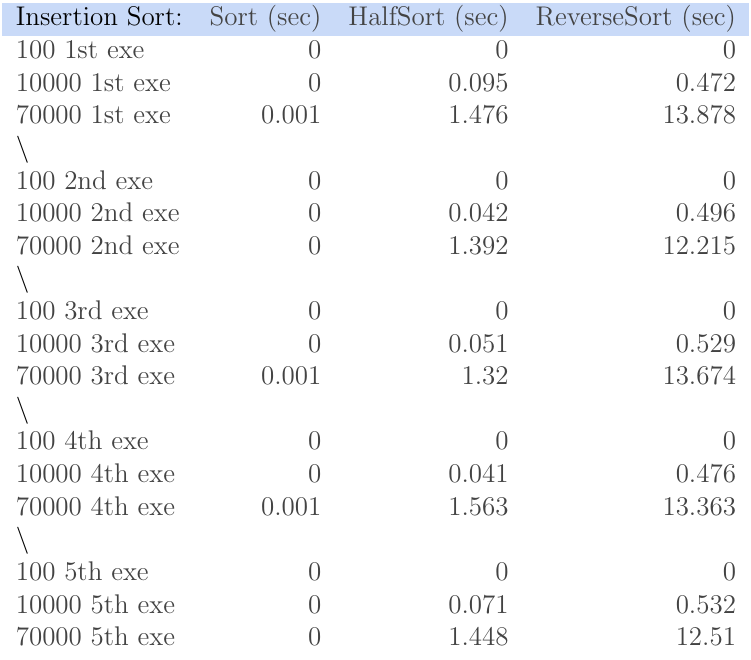
\includegraphics[scale=.7]{ISdatatable.PNG}
	\caption{Insertion Sort Data Table}
	\label{fig:mesh1}
\end{figure}
\begin{figure}[h]
	\centering
	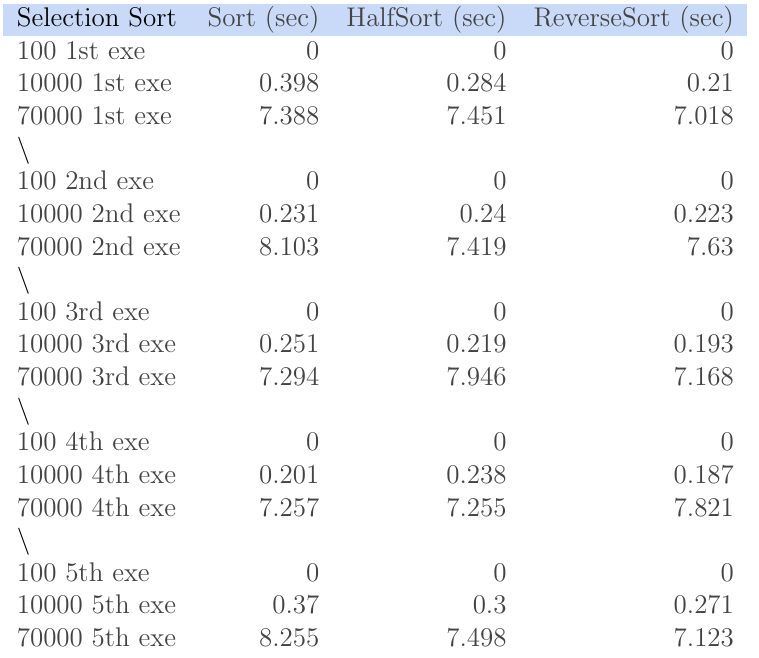
\includegraphics[scale=.7]{SSdatatable.PNG}
	\caption{Selection Sort Data Table}
	\label{fig:mesh1}
\end{figure}
\begin{figure}[h]
	\centering
	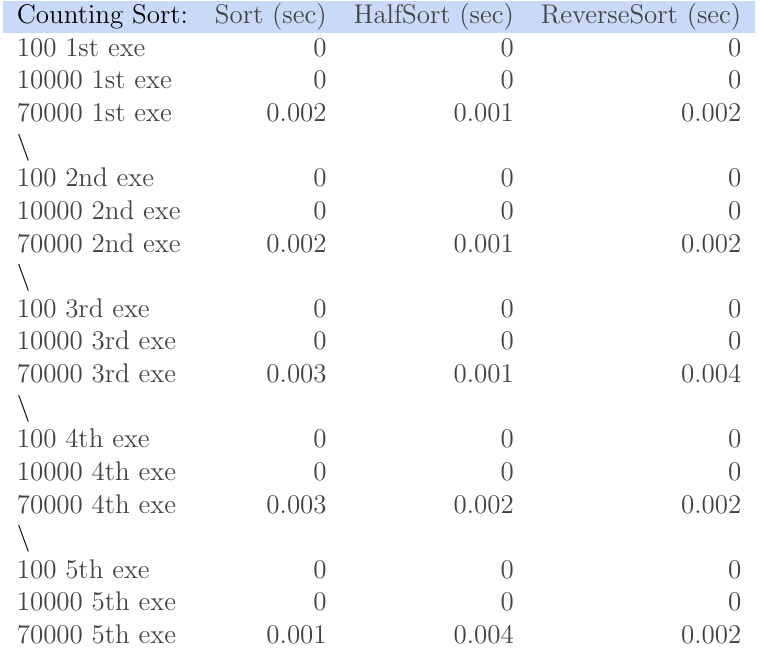
\includegraphics[scale=.7]{CSdatatable.PNG}
	\caption{Counting Sort Data Table}
	\label{fig:mesh1}
\end{figure}
\begin{figure}[h]
	\centering
	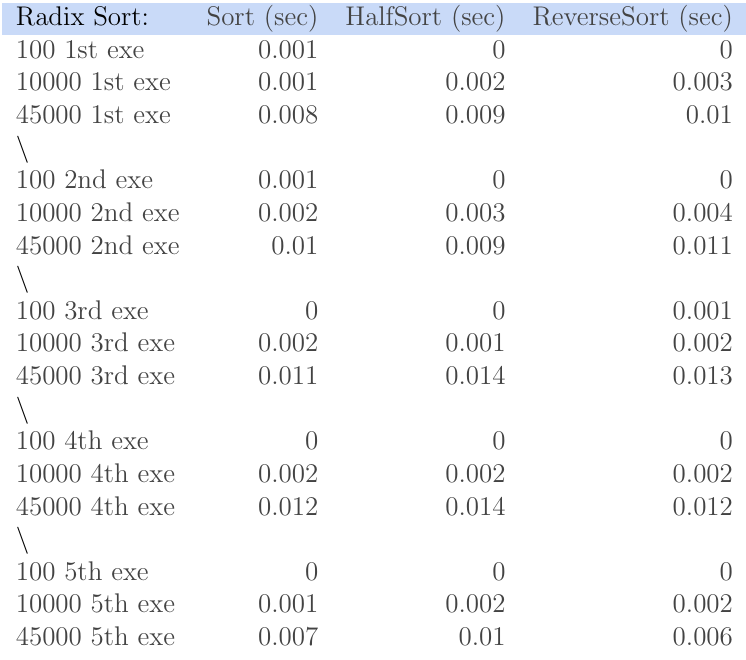
\includegraphics[scale=.7]{RSdatatable.PNG}
	\caption{Radix Sort Data Table}
	\label{fig:mesh1}
\end{figure}
\begin{figure}[h]
	\centering
	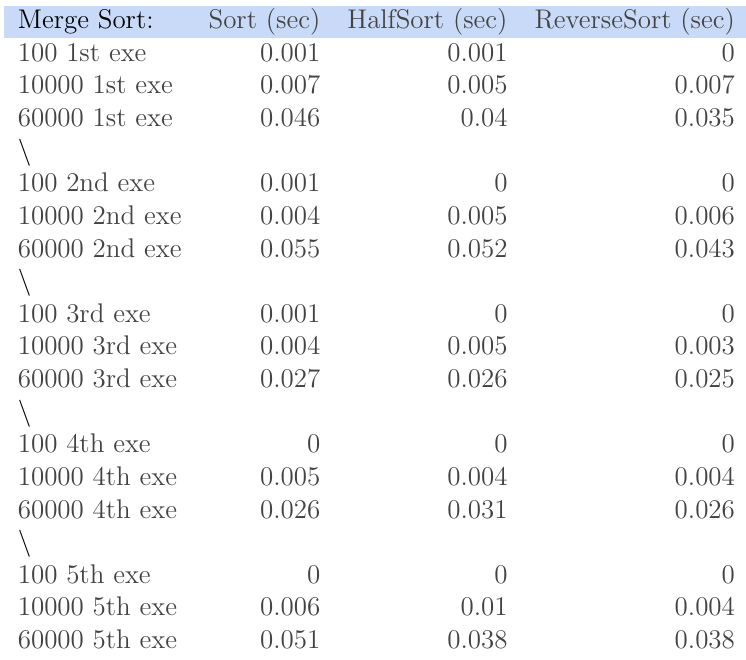
\includegraphics[scale=.7]{MSdatatable.PNG}
	\caption{Merge Sort Data Table}
	\label{fig:mesh1}
\end{figure}
\begin{figure}[h]
	\centering
	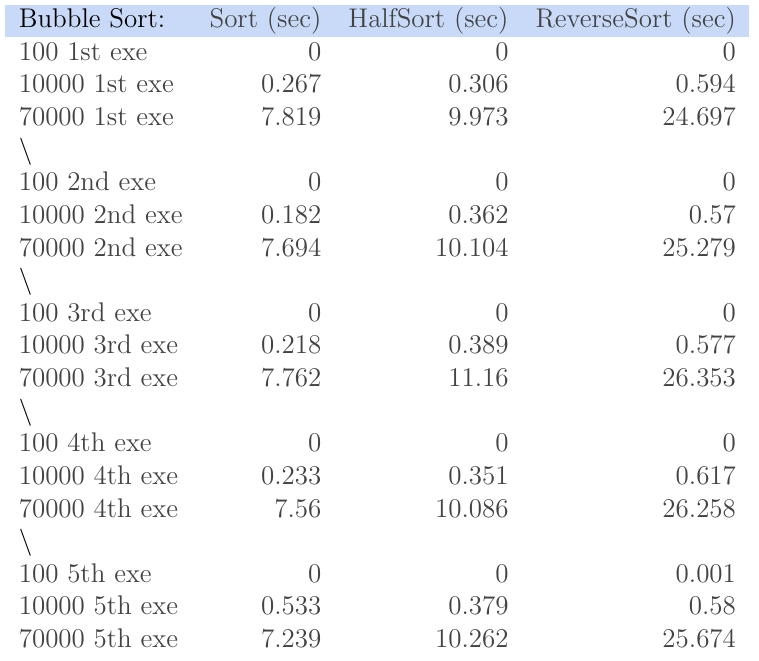
\includegraphics[scale=.7]{BSdatatable.PNG}
	\caption{Bubble Sort Data Table}
	\label{fig:mesh1}
\end{figure}
\begin{figure}[h]
	\centering
	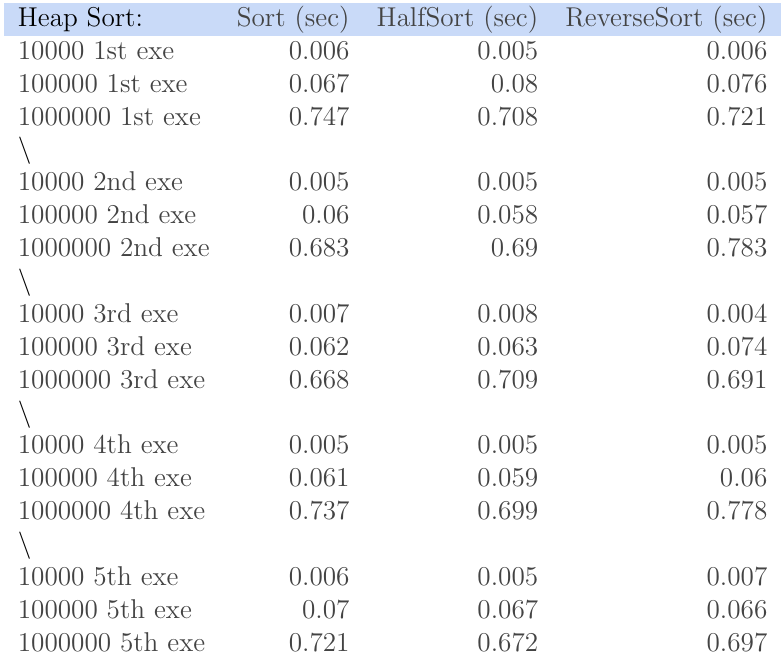
\includegraphics[scale=.7]{HSdatatable.PNG}
	\caption{Heap Sort Data Table}
	\label{fig:mesh1}
\end{figure}
\begin{figure}[h]
	\centering
	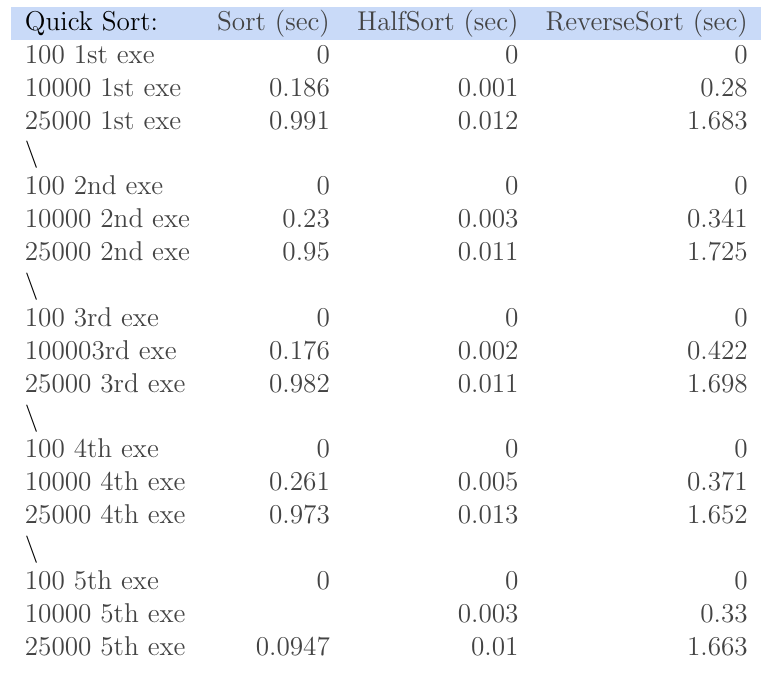
\includegraphics[scale=.7]{QSdatatable.PNG}
	\caption{Quick Sort Data Table}
	\label{fig:mesh1}
\end{figure}



\indent \\ \\ \\ \\\\\\\\\\\\\\\\\\\\\\\\\\\\\\\\\\\\\\ \\
\\\\\\\\\\\\\\\\\\\\\\\\\\\\\\\\\\\\\\\\\\\\\\\\\\\\\\\\\\\\\\\\\\\\\\\\\\\\\\\\\\\\\\\\\\\\\\\\\\\\\\\\\\\\\\\\\\\\\\\\\\\\\\\\\\\\\\\\\\\\\\\\\\\\\\\\\\\\\\
\section{Which of the five sorts seems to perform the best?}
\begin{figure}[h]
	\centering
	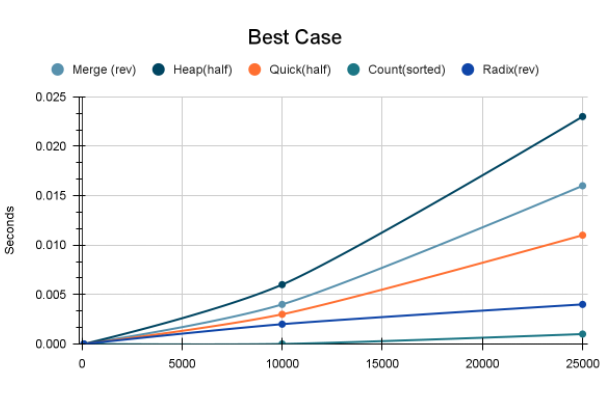
\includegraphics[width=\textwidth]{bestcase.PNG}
	\caption{Best Case Graph}
	\label{fig:mesh1}
\end{figure}
\begin{figure}[h]
	\centering
	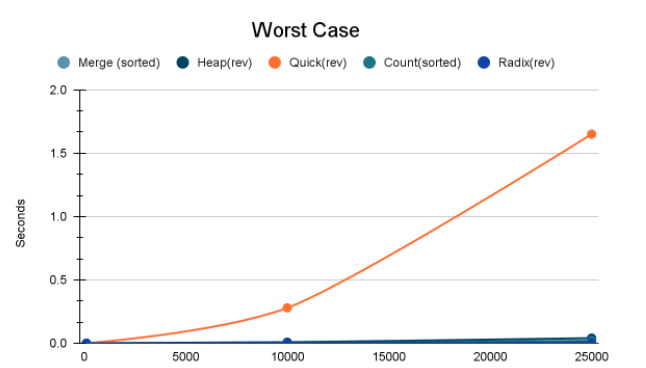
\includegraphics[width=\textwidth]{worstcase.PNG}
	\caption{Worst Case Graph}
	\label{fig:mesh1}
\end{figure}
\begin{figure}[h]
	\centering
	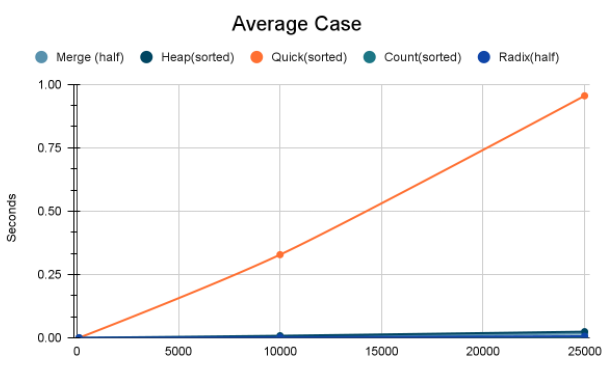
\includegraphics[width=\textwidth]{averagecase.PNG}
	\caption{Average Case Graph}
	\label{fig:mesh1}
\end{figure}
\indent \\\\\\\\\\\\\\\\\\\\\\\\\\\\\\\\\\\\\\\\\\\\\\\\\\\\\\\\\\\\\\\\\\\\\\\\\\\\\\\\\\\\
\subsection{The sort that perform the best}
Counting Sort performs the best in comparison to the other sorting algorithms which are the mergesort, heapsort, quicksort, and radix sort. Even when Quicksort at it’s best case performs O(nlogn) in addition with Merge and Heap. Counting Sort runs in linear time, resulting in it to be the quickest sorting algorithm. Taking in the input of a sorted array ranging from 100 to 25000 elements, Counting Sort outputs a running time no greater than 0.001 seconds. While Quicksort took in a half-sorted array to execute in it’s best case, it still ran at a time complexity of O(nlogn). Furthermore, Quicksort performance as seen from the graph and execution time performed the worst in comparison to the other sorts, O($n^2$) to be exact. Additionally, Counting Sort constantly remains the best in terms of running time in all three cases. In addition to that, Radix Sort as seen from the graph follows slightly behind Counting Sort. The time-complexity of Radix Sort is O(d*(n+k)) for all three cases. 
\indent \\\\
\section{To what extent do the best, average and worst-case analyses of each sort agree with the experimental results?}

\begin{figure}[h]

	\centering
	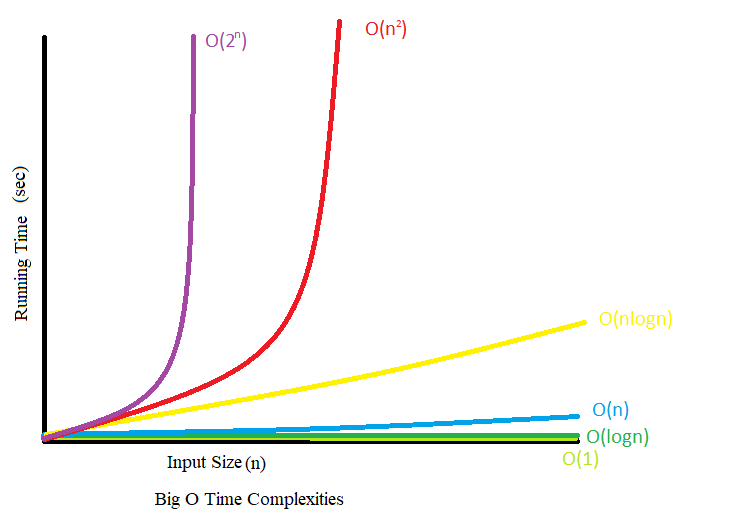
\includegraphics[width=\textwidth]{Asymptotic Notations.PNG}
\caption{Asymptotic Notations}
    \label{fig:mesh1}
\end{figure}
	The graph above, Big O Time Complexities, will be used to compare how the graphed experimental results relate to the actual expected worst cast, best case, and average case of each sorting algorithm. For each sorting algorithm, the reversed input array line will correspond to the worst case, the half-sorted array line will correspond to the average case, and the already sorted  array line will correspond to the best case.\\
\\
\\


	\subsection{Insertion Sort:}

	As previously mentioned, the worst case, best case, and average case analysis for Insertion Sort are as follows: \\	

	Best Case: O(n) - Sorted Array\\
	\indent Average Case: O($n^2$) - Random Order Array\\
	\indent Worst Case: O($n^2$) - Reversed Array\\
\begin{figure}[h]
	\centering
	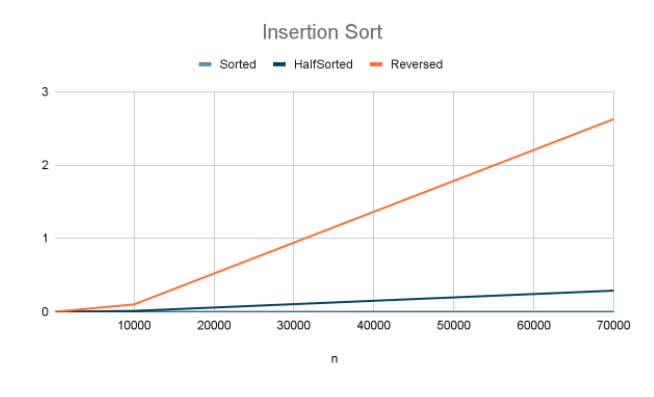
\includegraphics[width=\textwidth]{Insertion Graph.PNG}
\caption{Insertion Sort Graph}
    \label{fig:mesh1}
\end{figure}

	The reversed array input results in the worst case for the Insertion Sort algorithm which is O($n^2$). The orange line, which is from the reversed input array, corresponds to the worst case. When comparing it to O($n^2$) in the Big O Time complexities graph it appears to agree with the worst case analysis of Insertion Sort  which as is known, is O($n^2$). As the input size increases the running time increases quadratically.\\ 
\\
\indent The dark blue line from the half-sorted array is also expected to be O($n^2$) because it corresponds to the average case which as is known is also O($n^2$). However, when comparing the Half Sorted line to the O($n^2$) line in the Big O Time complexities graph they do not appear to be the same. In fact, the Half Sorted line appears to relate more closely to the O(nlogn) line. When it comes to the average case, the experimental results do not appear to agree with the expected time analysis of O($n^2$). The reason for this is most likely due to the fact that the array is already half sorted. As is known the time of insertion sort for an already sorted array is O(n) which is a bit faster than O($n^2$). Knowing this, it is clear that the algorithm ran quicker through the first half of the array than it did in the reversed array. If the array were truly random as expected for the average case, then time complexity would most likely correspond to the expected O($n^2$). Of course, there is an argument to be made that a half sorted array is within the realm of possibilities when it comes to randomly ordered arrays. So, when it comes to whether or not the average case of Insertion Sort agrees with the experimental results that were derived, the answer is that it depends on how truly random the array is.\\ 
\indent	Moving on to the best case of Insertion Sort, the already sorted array line is a flat line all the way across the board. This appears to be completely in line with O(n) on the Big O Time complexities graph. As previously mentioned the expected best case of Insertion Sort is O(n) or linear time, which occurs when the input is in an already sorted order. This means that the algorithm will only do n comparisons. So when it is given a sorted array of size 70000, it will do 70000 comparisons, whereas in the worst case when given the same 70000 sized array but in reverse order, it will do 4,900,000,000 comparisons. As such, the running time for an already sorted array should have a much lower increase as the input size grows than the worst case. This is clearly reflected in the experimental graph. When it comes to the best case of insertion sort, the experimental data appears to completely agree with the asymptotic analysis for the best case of Insertion Sort which is O(n).\\
\\
\\
\\
\\
\\
\\
\\

	\subsection{Selection Sort:}

	As previously mentioned, the worst case, best case, and average case analysis for Selection Sort are as follows: \\

	\indent	Best Case: O($n^2$) - Sorted Array\\
	\indent	Average Case: O($n^2$) - Random Order Array\\
	\indent	Worst Case: O($n^2$) - Reversed Array\\
	
\begin{figure}[h]
	\centering
	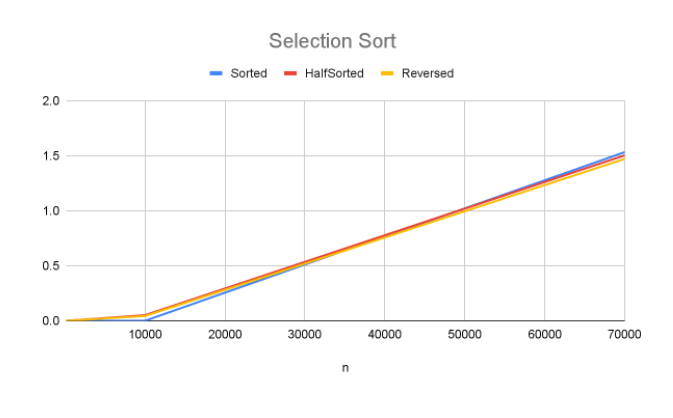
\includegraphics[width=\textwidth]{Selection Graph.PNG}
\caption{Selection Sort Graph}
    \label{fig:mesh1}
\end{figure}

	Regarding Selection Sort, the worst, best, and average case analysis are all O($n^2$). Knowing this, one can reasonably expect the experimental results of each array to be very close when graphed and also correspond to the O($n^2$) curve shown in the Big O Time Complexities graph. As can be seen from the Selection Sort graph above which shows the experimental results, each line is indeed very close and similar in the way the execution time increases as the input size increases. This clearly indicates that the algorithm had a very similar execution time for the reverse order array, the half-sorted array, and also the sorted array. The execution times for each array also appear to increase quadratically as the input sizes increase similar to O($n^2$) on the Big O Time Complexities graph. One can safely say that in the case of Selection Sort, the experimental results agree with the best, average and worst-case analysis.\\
	
	\subsection{Bubble Sort:}

	As previously mentioned, the worst case, best case, and average case analysis for Bubble Sort are as follows: \\

	\indent Best Case: O(n) - Sorted Array\\
	\indent	Average Case: O($n^2$) - Random Order Array\\
	\indent	Worst Case: O($n^2$) - Reversed Array\\

\begin{figure}[h]
	\centering
	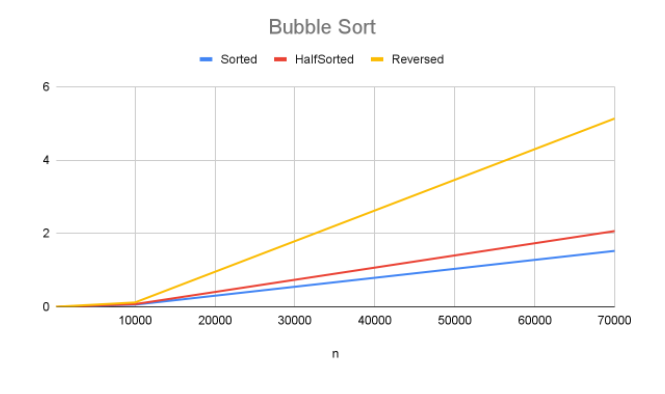
\includegraphics[width=\textwidth]{Bubble Sort.PNG}
\caption{Bubble Sort Graph}
    \label{fig:mesh1}
\end{figure}

	
	To begin, it must be mentioned that the worst case, best case, and average case analysis for Bubble Sort is the same as the worst case, best case, and average case analysis for Insertion Sort. As such, one can expect very similar experimental results to those seen with the Insertion Sort algorithm. The reversed line in the Bubble Sort graph is very similar to that seen in the Selection Sort graph. Similarly, as the input size grows, the execution times appear to grow quadratically. Furthermore, when comparing the reversed line to the O($n^2$) line on the Big O Time Complexities graph, the reversed line has a dramatic increase as the input size grows which corresponds to O($n^2$). It can safely be said that in the worst case of Bubble sort, the experimental results agree with the worst case analysis. \\
\indent	Moving on to the average case, something strange happens. The half-sorted line, which corresponds to the average case, and the sorted line, which corresponds to the best case, are very close in their execution times over input sizes. Similar to Insertion Sort, the average case appearing faster than the expected O($n^2$) can be attributed to the fact that the input was a half sorted array. Again, an argument can be made that a half sorted array is a possibility in random arrays. For the average case, the experimental results do not appear to agree with the average case analysis. However, if each execution time was doubled to account for the half of the array that was sorted, it is certain that the line would be very close to that of the worst case. Thus, it can be said that the experimental results may agree with average case analysis if the array was in a truly randomized order, but even then the results may vary in the way that they could be even faster or slower. \\
\indent As for the best case, once again something strange happens. When comparing the sorted line from the Bubble Sort graph to the Big O Time Complexities graph, it appears to correspond more similarity to the O(nlogn) line rather than the expected O(n) line. The sorted line should also be similar to the best case sorted line seen in the Selection Sort graph. Once again this is not the case. So what did happen? To explain this the Pseudo-Code of the utilized Bubble Sort algorithm will be shown below.\\

SKbubbleSort (A, n)\\
\indent\indent	for i ← 1 to n\\
\indent\indent\indent		for j ← 0 to n - i\\
\indent\indent\indent\indent			if A[j] $>$ A[j + 1]\\
\indent\indent\indent\indent\indent				Do A[j] $\longleftrightarrow$ A[j + 1]\\

\indent	In order to get the best case from an already sorted array, Bubble Sort needs some sort of flag to remember if any swapping has actually occurred. With such a flag in place, if no swapping occurred then the algorithm will quickly know that the array is already sorted and will quit after at most the second iteration. If the algorithm utilized in the experiment had something like a boolean to check if swapping has occurred then the experimental results would probably agree with the best case analysis, however in the case of the Bubble Sort algorithm above, the experimental results do not agree with the best case analysis of O(n) and seem to more closely correspond to O(nlogn).\\

	\subsection{Merge Sort:}
	
	\indent\indent Best Case: O(n log n) - Sorted Array\\
	\indent Average Case: O(n log n) - Random Order Array\\
	\indent Worst Case: O(n log n) - reversed Array\\	

\begin{figure}[h]
	\centering
	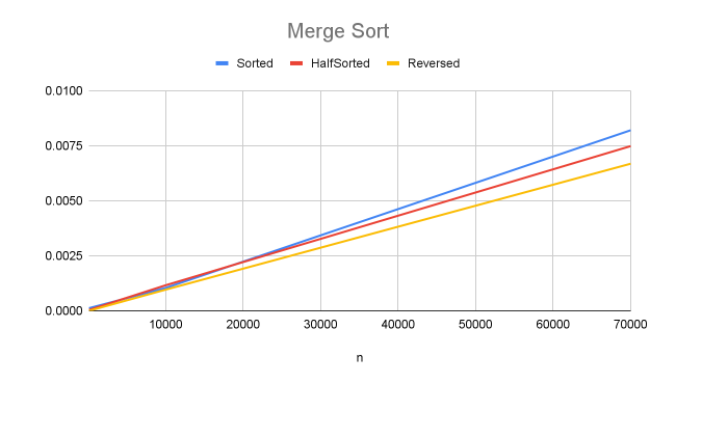
\includegraphics[width=\textwidth]{Merge Sort.PNG}
\caption{Merge Sort Graph}
    \label{fig:mesh1}
\end{figure}

	Regarding Merge Sort, the best, worst, and average case analysis are all O(nlogn). This means that one can reasonably expect that the Sorted, Half Sorted, and Reversed lines will appear very similar when graphed in their relation of execution times over increasing input sizes.. As can be seen in the Merge Sort graph above, this appears to definitely be the case. Furthermore, when comparing each line to the O(nlogn) line in the Big O Time Complexities graph, they appear to perfectly coincide. In the case of Merge Sort it is overwhelmingly clear that the best, average and worst-case analyses agree with the experimental results.\\
\indent \\\\\\\\\\\\\\\\\\
\section {Is The Number of Comparisons A Good Predictor of the Execution Time?}

\subsection{Insertion Sort Correlation} 

\begin{figure}[H]
	\centering
	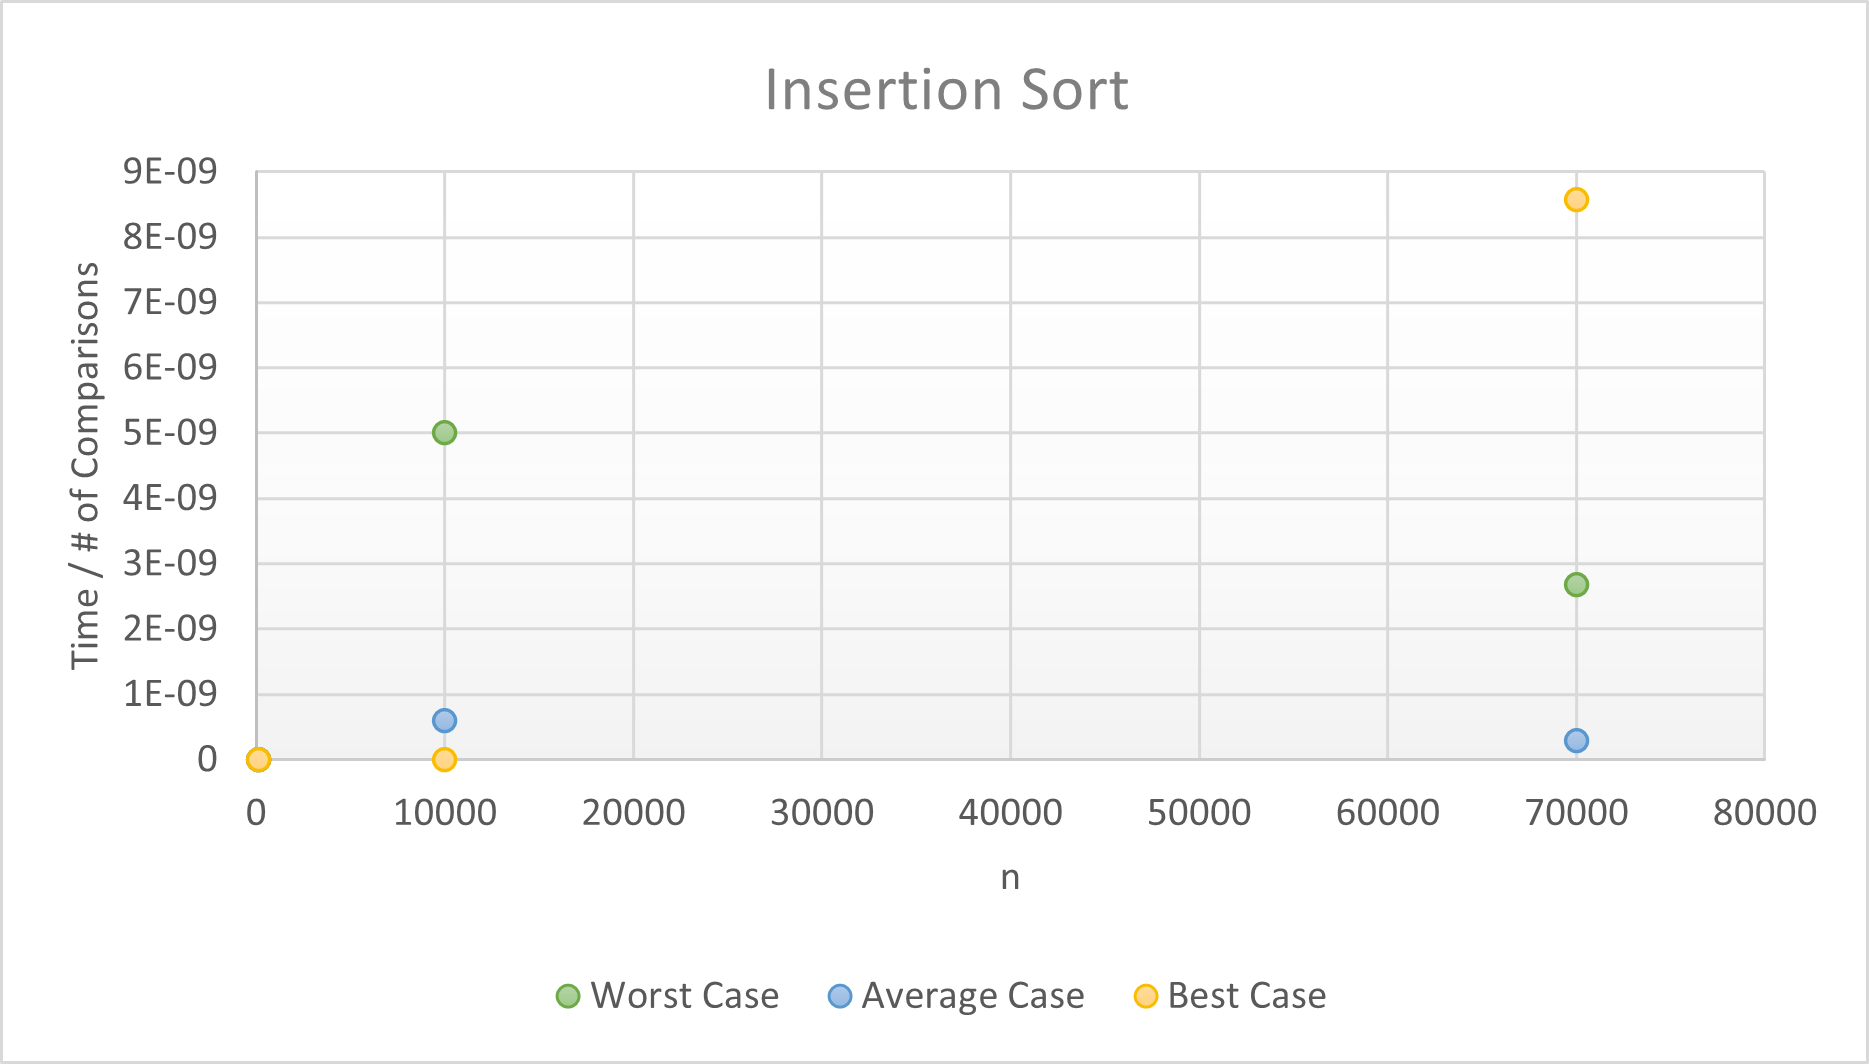
\includegraphics[width=\textwidth]{Icorr.png}
\caption{Insertion Sort Data Correlation}
    \label{fig:mesh1}
\end{figure}

	Regarding Insertion Sort, in Figure 12, there appears to be a small positive correlation between the execution time divided by the number of comparisons vs n when n is less than or equal to 10000. However that correlation becomes a weak positive correlation as the n grows.\\
\\
\\
\\
\\
\\
\\

\subsection{Selection Sort Correlation} 
\begin{figure}[H]
	\centering
	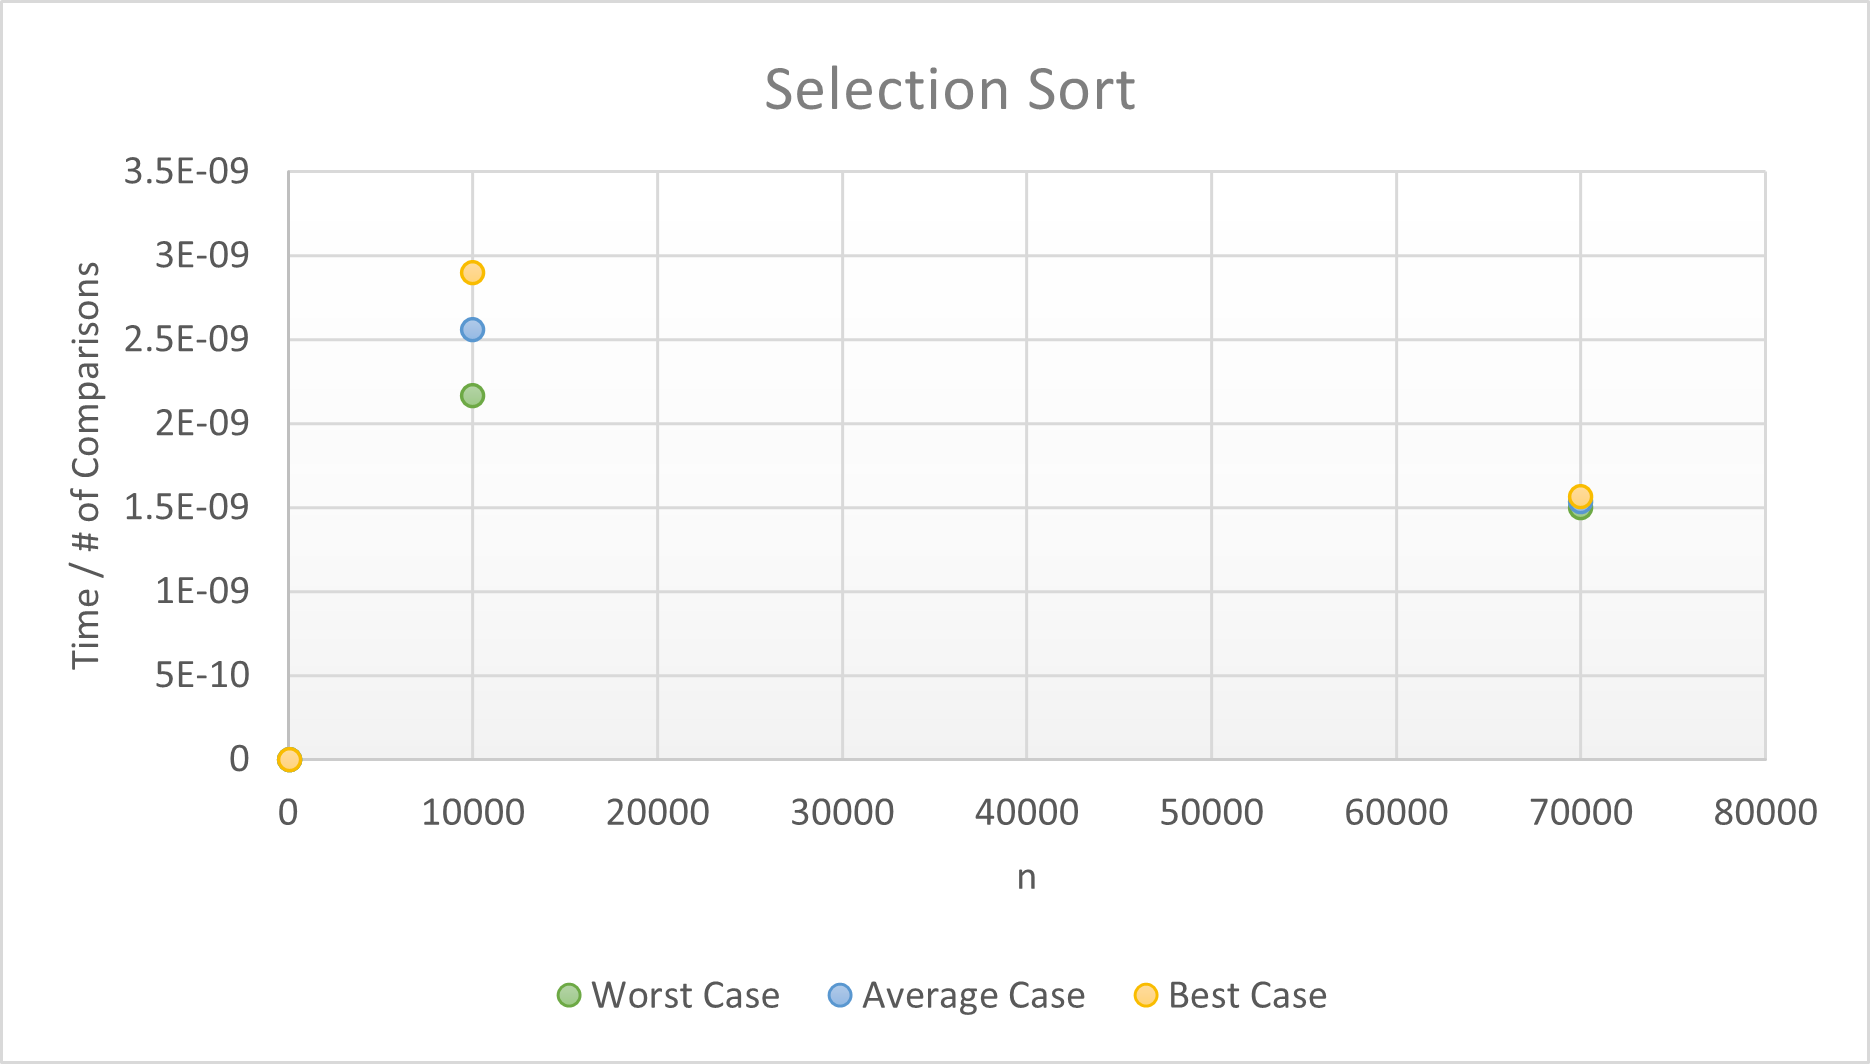
\includegraphics[width=\textwidth]{Scorr.png}
\caption{Selection Sort Data Correlation}
    \label{fig:mesh1}
\end{figure}

	Regarding Selection Sort, in Figure 13, there does appear to be a Curvilinear correlation between the execution time divided by the number of comparisons vs n.\\
\\
\\
\\
\\
\\
\\
\\
\\
\\\\\\\\
\subsection{Bubble Sort Correlation} 
\begin{figure}[h]
	\centering
	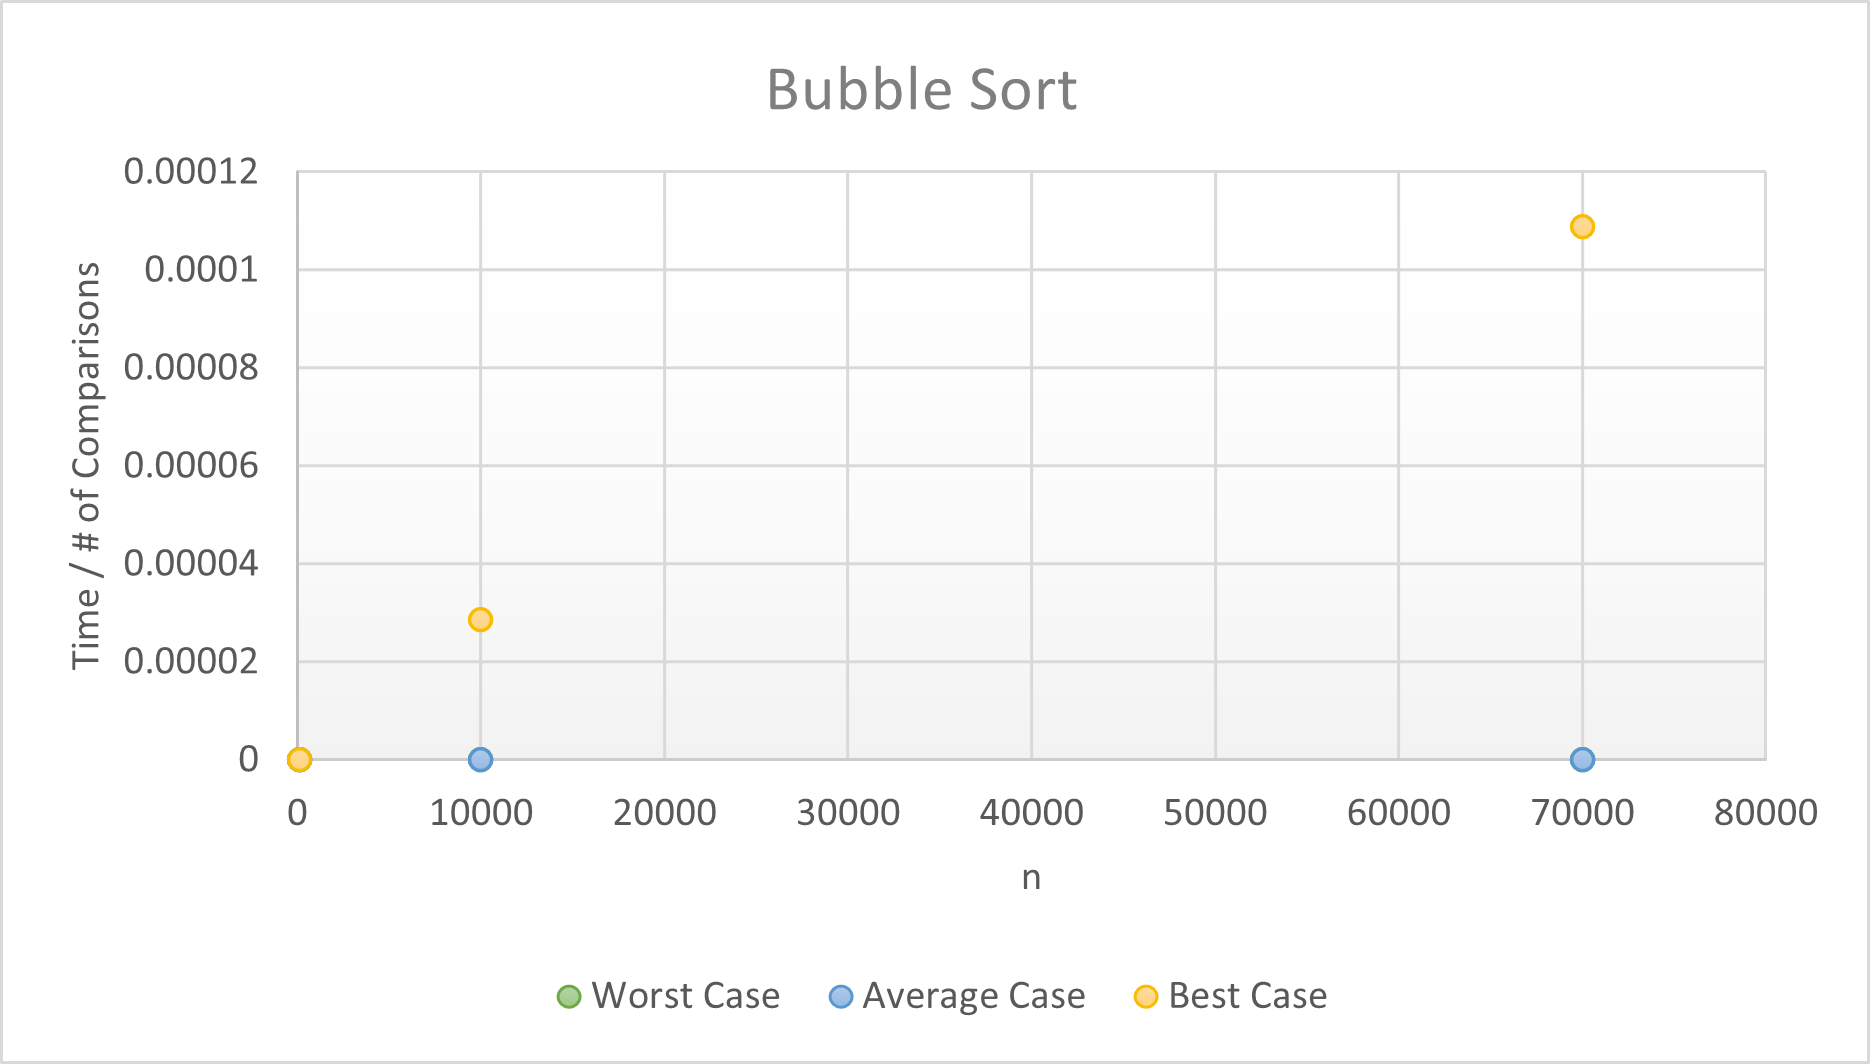
\includegraphics[width=\textwidth]{Bcorr.png}
\caption{Bubble Sort Data Correlation}
    \label{fig:mesh1}
\end{figure}

	Regarding Bubble Sort, in Figure 14, there does appear to be a weak positive correlation.\\
\\
\\
\\
\\
\\
\\
\\
\\
\\
\\
\\\\\\\\
\subsection{Merge Sort Correlation} 
\begin{figure}[h]
	\centering
	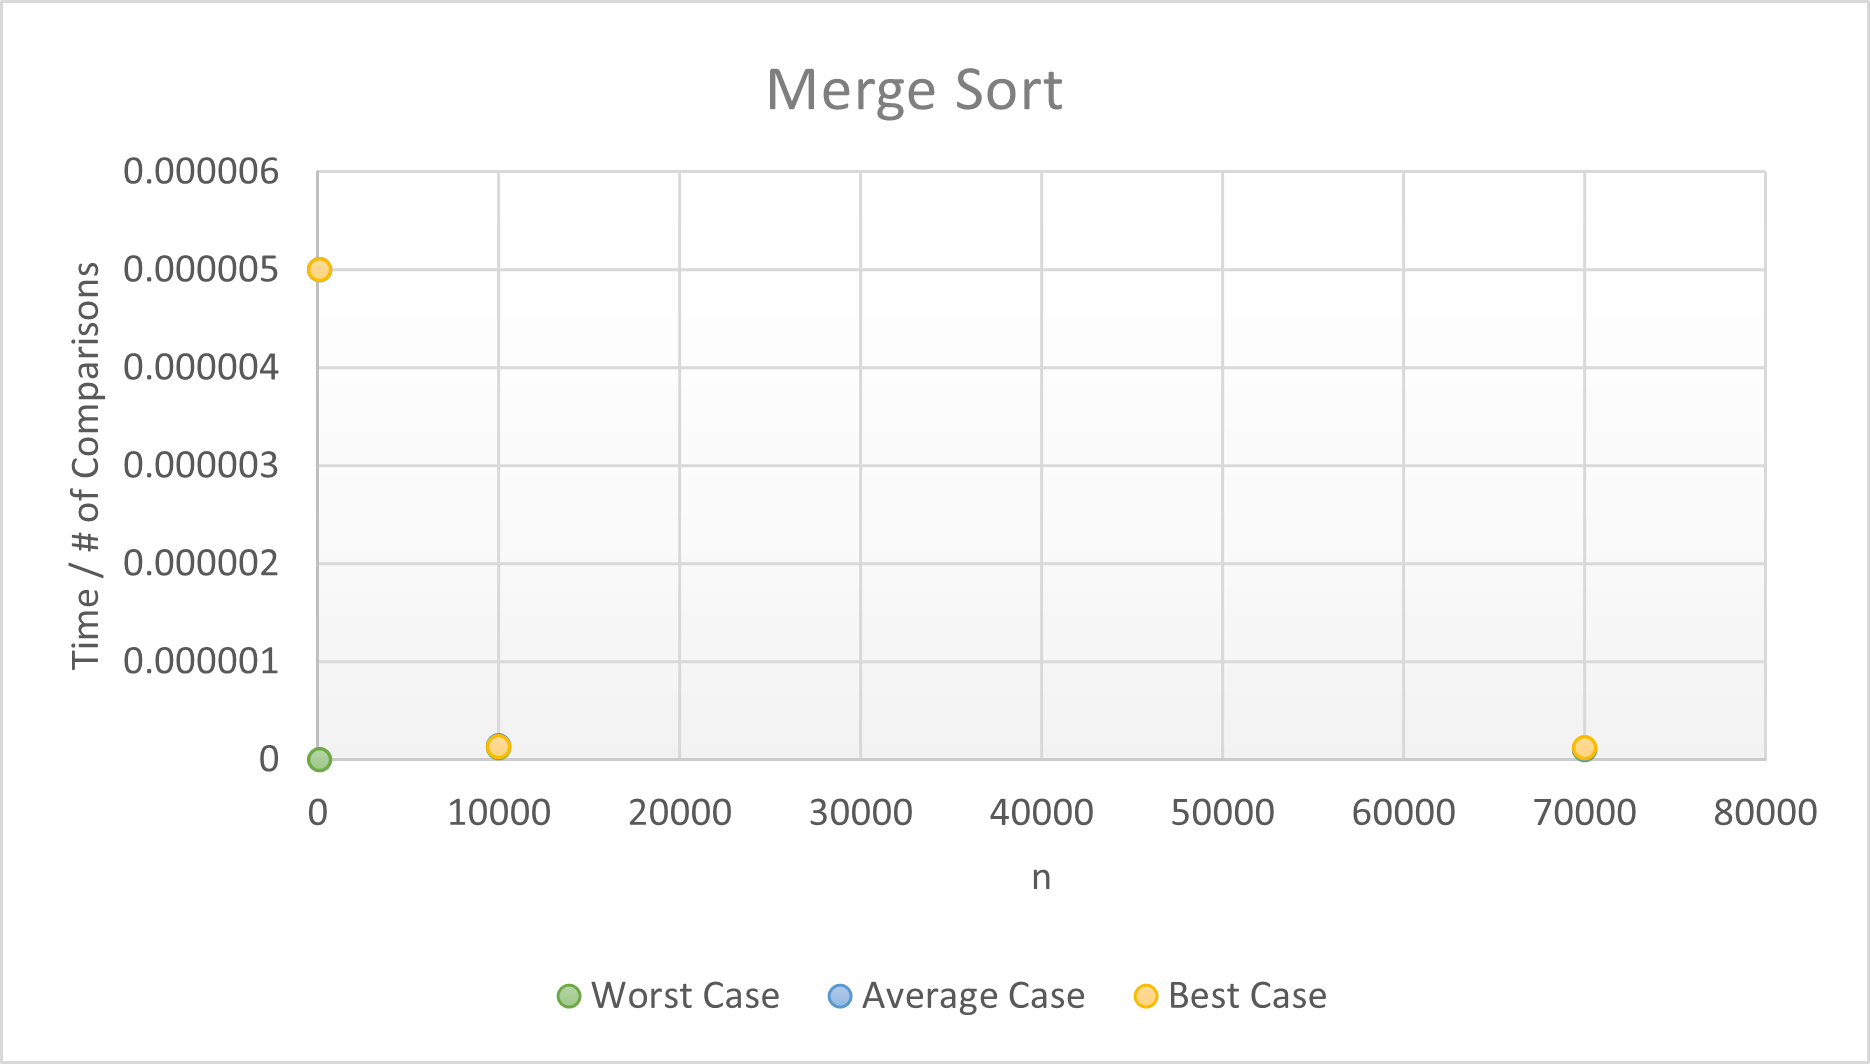
\includegraphics[width=\textwidth]{Mcorr.png}
\caption{Merge Sort Data Correlation}
    \label{fig:mesh1}
\end{figure}
	Regarding Merge Sort, in Figure 15, it could be argued that there is a very weak negative correlation. However, there also appears to be no correlation at all.\\
\\
\\
\\
\\
\\
\\
\\
\\
\\
\\
\\
\\
\\
\\
\subsection{Heap Sort Correlation} 
\begin{figure}[h]
	\centering
	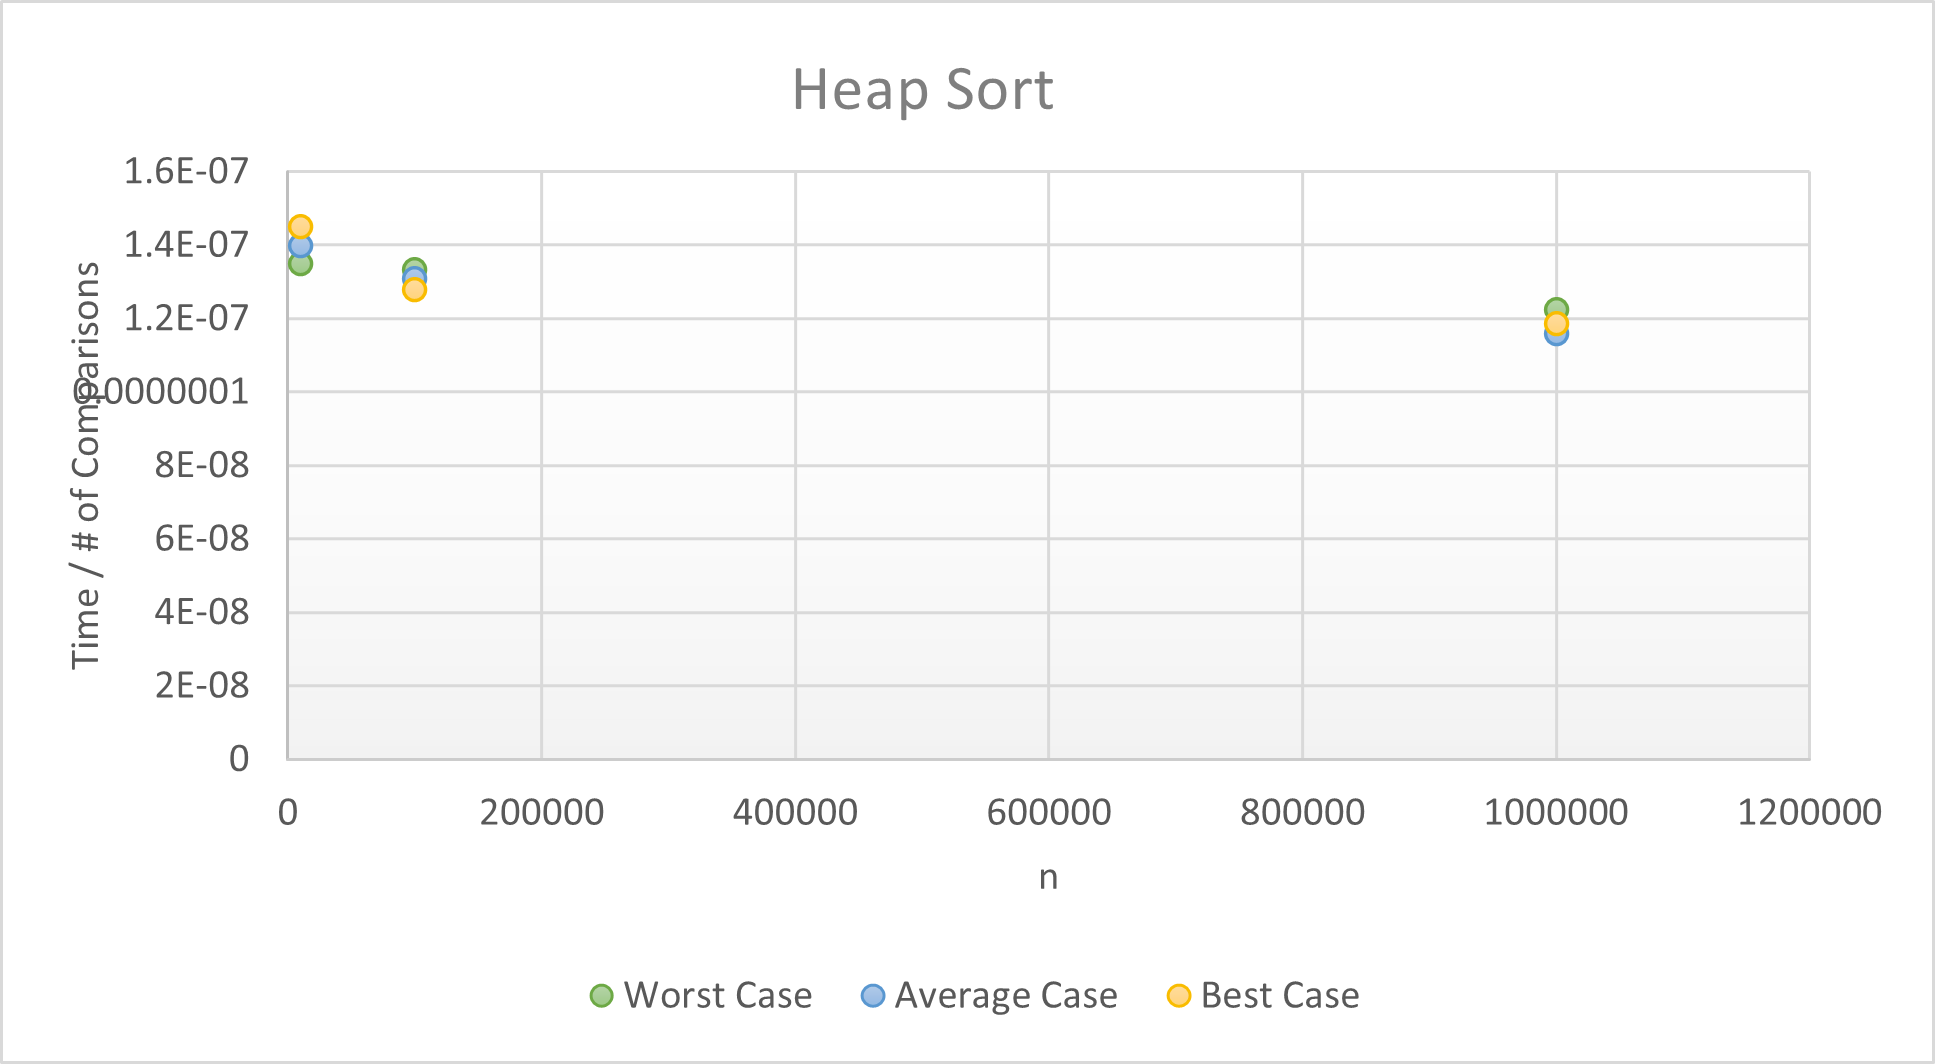
\includegraphics[width=\textwidth]{Hcorr2.png}
	\caption{Heap Sort Data Correlation}
	\label{fig:mesh1}
\end{figure}
Regarding Heapsort, in Figure 21, similar to Selection Sort there appears to be a Curvilinear correlation.
\indent
\\
\\
\\
\\
\\
\\
\\
\\
\\
\\
\\
\\
\\
\\
\subsection{Quick Sort Correlation} 
\begin{figure}[h]
	\centering
	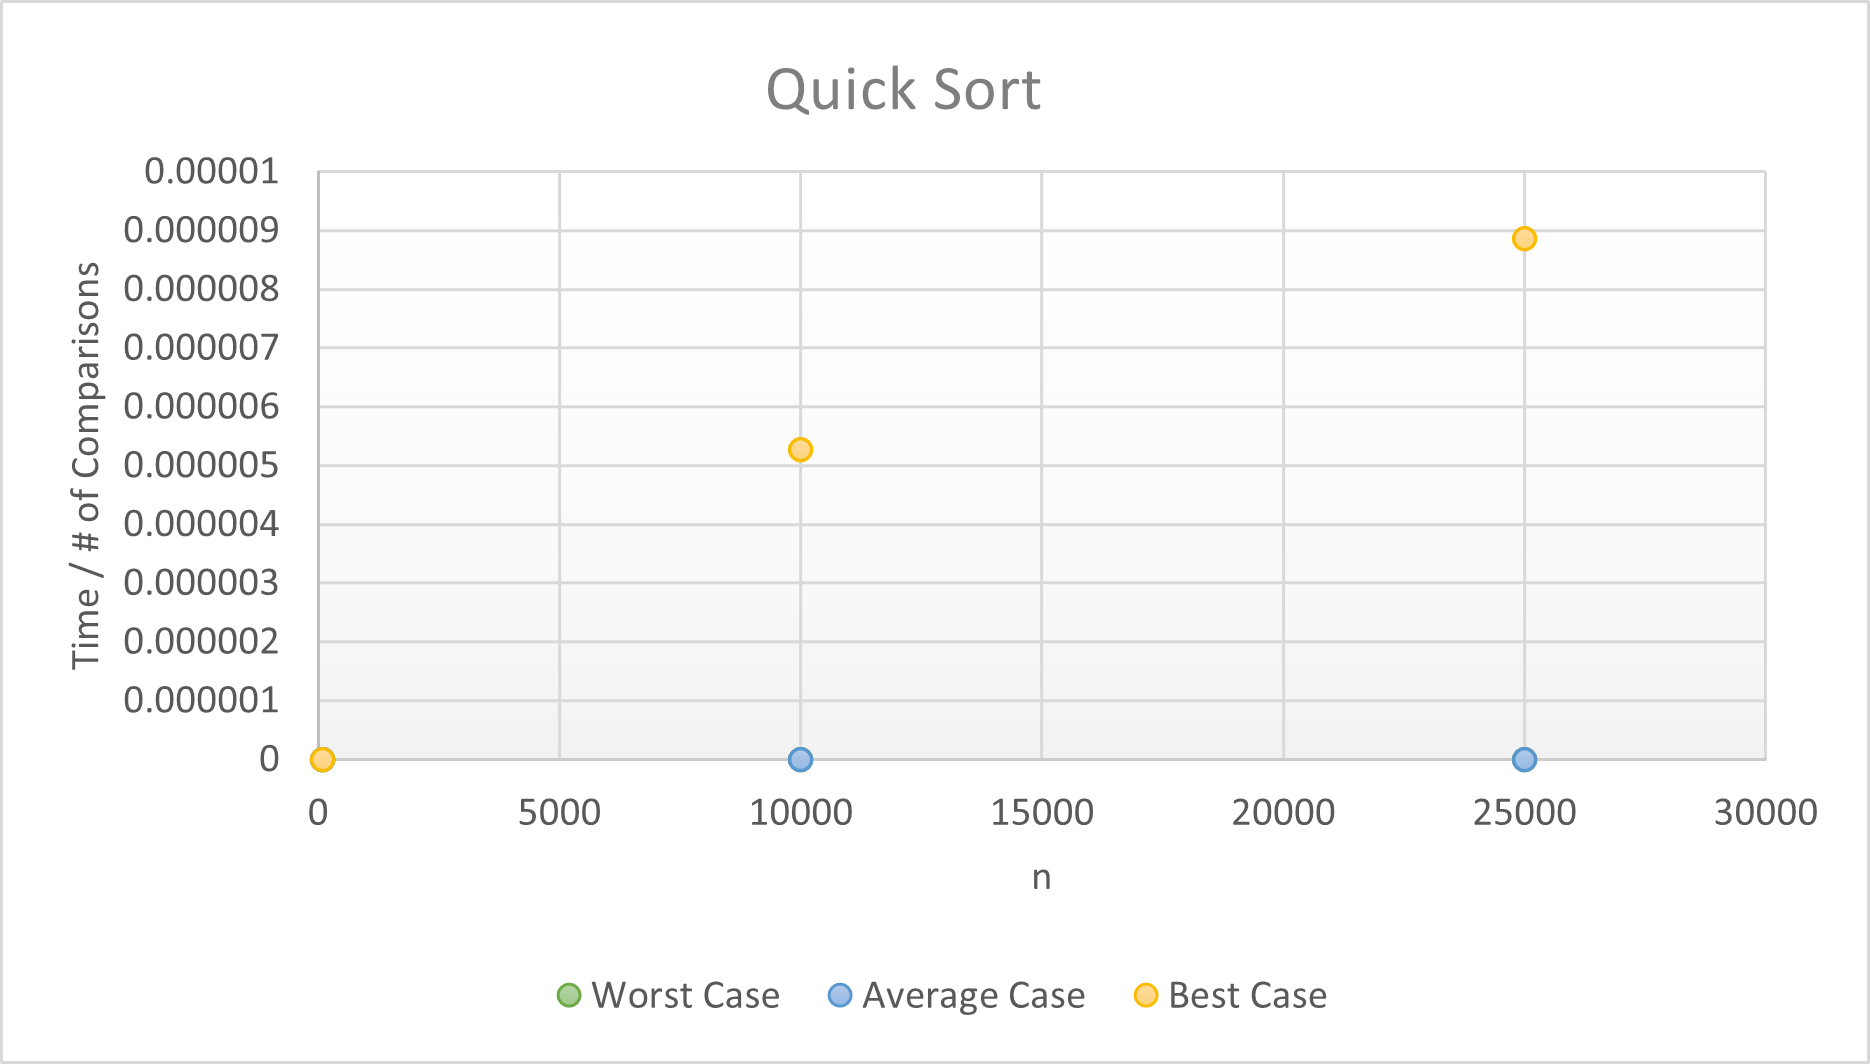
\includegraphics[width=\textwidth]{Qcorr.png}
	\caption{Quick Sort Data Correlation}
	\label{fig:mesh1}
\end{figure}
Regarding Quicksort, in Figure 22, there appears to be a weak positive correlation. Although it is a weak correlation, the data points are evenly spread indicating that a relationship does exist.
\subsection{Conclusion}

	To answer the question, is the number of comparisons truly a good predictor of execution times? For each comparison sorts scatter plot of the execution time divided by the number of comparisons vs n, there appears to be some form of correlation. For Insertion Sort, there was a weak positive correlation, for Selection Sort there was a curvilienar correlation, for Bubble Sort there a weak positive correlation, and finally for Merge Sort there was a very weak negative correlation. Although these correlations are weak they are present. These correlations would also most likley become stronger with more data sizes if they follow the trend of each comparison sorts correlation. To conclude, the number of comparisons is a good predictor of execution times.

\indent\\
	\section{Part 2: Brute/Inefficient method}
	The brute/inefficient method of finding all the pairs/elements equal to the sum.
	\subsection{PseudoCode}
	ALG: BruteSum(A,n,x) \\
	\indent \indent total←0     \\
	\indent \indent for i←0 to n \\
	\indent \indent \indent for a←i to n \\
	\indent \indent \indent \indent do sum←A[i]+A[a] \\
	\indent \indent \indent \indent do if sum==x \\
	\indent \indent \indent \indent \indent \indent total ++ \\
	\subsection{Running time analysis}
	ALG: BruteSum(A,n,x) \\
	\indent \indent total←0 \indent \indent \indent \indent \indent \indent \indent -1   \\
	\indent \indent for i←0 to n \indent \indent \indent \indent \indent \indent -n+1\\
	\indent \indent \indent for a←i to n \indent \indent \indent \indent \indent -n+1\\
	\indent \indent \indent \indent do sum←A[i]+A[a] \indent \indent  -n\\
	\indent \indent \indent \indent do if sum==x \indent \indent \indent -1 \\
	\indent \indent \indent \indent \indent \indent total ++ \indent \indent \indent -1\\ \\
	1+n+n+n+1+1= \\
	Removing Constants: \\
	(n)+(n)+n \\
	Keeping the highest order term which there are two: \\
	The time complexity is O($ n^2 $) \\
	\subsection{Report of brute/inefficient method}
	\indent \indent The algorithm takes A for the list of array and n is taking the size of it while x is the value that we need to find the sum for. The total is to figure out if there is at least one sum that is found and the running time would be constant. The first for loop would start at the first element of the array list and then would go into the next for loop which would be considered a nested loop. The first for loop running time would be n+1 as it will go through the whole list. As soon as the second loop starts going through the function it will check to see if there is a sum that we are looking for. \\
	\indent The function is added from the first element and while the second element is going through the list and being added with the first element of the array to see if the sum is found. The time for this would n as it will continue to be active as the second for loop keeps going through the list. The if list is to see if the sum is found and would just be a constant as it isn’t always executed and within the if function the total is being added by one which is also a constant. After the second for loop is done then the first loop will go onto the next element and repeat the second for loop from a new starting point from the first for loop. Which will give the time complexity of the function o($n^2$) because of the two for loops.
	
	\section{Part 2: Efficient method}
	The efficient method of finding all the pairs/elements equal to the sum.
	\subsection{PseudoCode}
	ALG: SUM-CHECK(A, x, n) \\
	\indent \indent found\_pair←false     \\
	\indent \indent unordered\_set HashTable \\
	\indent \indent \indent for i←0 to n \\
	\indent \indent \indent \indent do y← x - A[i] \\
	\indent \indent \indent \indent do if HashTable.find(y)  != HashTable.end() \\
	\indent \indent \indent \indent \indent \indent then do if A[i] + y = x \\
	\indent \indent \indent \indent \indent \indent \indent then found\_pair ← true \\
	\indent \indent \indent \indent \indent \indent \indent return found\_pair \\
	\indent \indent \indent HashTable.insert(i) \\
	\subsection{Running time analysis}
	ALG: SUM-CHECK(A, x, n) \\
	\indent \indent found\_pair←false \indent \indent \indent \indent \indent \indent \indent \indent \indent \indent \indent \indent \space{-n}\\
	\indent \indent unordered\_set HashTable\indent \indent \indent \indent \indent \indent \indent \indent \indent \indent \space{-1}  \\
	\indent \indent \indent for i←0 to n \indent \indent \indent \indent \indent \indent \indent \indent \indent \indent \indent \indent \space \space \space{-n + 1}  \\
	\indent \indent \indent \indent do y← x - A[i] \indent \indent \indent \indent \indent \indent \indent \indent \indent \indent  \indent-n \\
	\indent \indent \indent \indent do if HashTable.find(y)  != HashTable.end() \indent \indent \space \space -1\\
	\indent \indent \indent \indent \indent \indent then do if A[i] + y = x \indent \indent \indent \indent \indent \indent \space \space-n\\
	\indent \indent \indent \indent \indent \indent \indent return true \indent \indent \indent \indent \indent \indent \indent \indent \indent -n \\
	\indent \indent \indent HashTable.insert(i) \indent \indent \indent \indent \indent \indent \indent \indent \indent \indent \space \space\space -1\\
	\indent \indent return false\indent \indent \indent \indent \indent \indent \indent \indent \indent \indent \indent \indent \indent \indent - n \\
	= n + 1 + (n + 1) + n + 1 + n + n  + 1 + n   \\
	= n + 1 + n + 1 + n + 1 + n + n + 1 + n\\
	= 6n + 4\\
	Removing Constants: \\
	= n \\
	Keep the highest order term: n \\
	The time complexity is O($ n $) or Linear time \\
	\subsection{Report of Efficient method}
	\indent \indent The algorithm SUM\-CHECK takes a vector or array A, an integer x, which is the sum, and an integer n which is the size of A. A is a vector of type integer that holds a list of numbers. x is the desired sum that the algorithm will check if vector A has a pair that sums to x. First a boolean called “found\_pair” is initialized to false. This boolean will be used to return true if a pair is found or return false if a pair is not found. Then an empty unorderd\_set named “HashTable” is created. Next, a for loop will go through each element in vector A starting from element at index 0 to element at index n. A new integer y will then be set to the difference of x and the current element at element A[i]. At this point, y is a possible half of the pair needed to sum to x. The next part of the algorithm will check if the HashTable contains the other needed number. Moving on, An if statement will then check if the unordered\_set contains this half of the possible pair by utilizing the .find() function which either returns an iterator to the found element or an iterator to .end(). Then the algorithm will then add y to the current element A[i] from the for loop to check if y and A[i] sums to x. If it does sum to x then a pair exists in A and the algorithm will set found\_pair to true and return. If y and A[i] does not sum to x then the algorithm will insert A[i] into the undordered\_set. This process will repeat until each element in A[i] has been checked and a pair has not been found or until a pair is found. This results in a time complexity of O(n).
\\
\\




\end{document}